\subsection{Labels Tab}
\label{sec:geoview_labels_tab} 
 
\begin{figure}[H]
   \center
    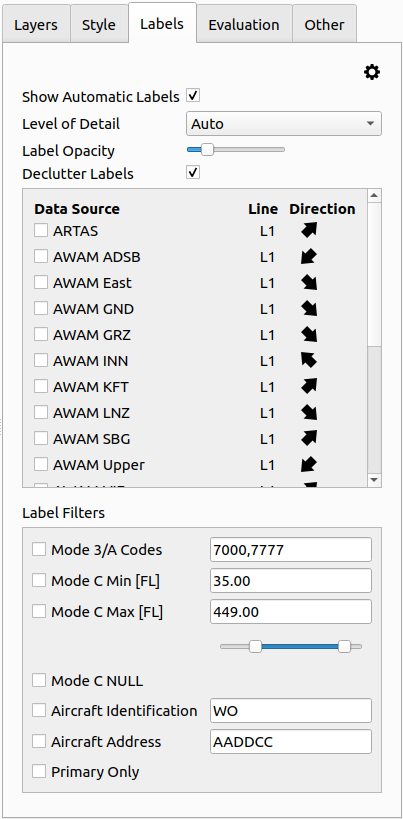
\includegraphics[width=8cm,frame]{figures/geoview_labels_tab.png}
  \caption{Geographic View Labels tab}
\end{figure}

In the 'Labels' tab, several elements exist:

\begin{itemize}
 \item \includegraphics[width=0.5cm,frame]{../../data/icons/edit.png} button: Label menu 
 \item Auto Label Checkbox: Toggles auto-label feature
 \item Level of Detail: What level of detail should be used for labels
 \item Data Sources: Selects which data sources to label and label direction
 \item Label Filters: Filters which targets are labeled
\end{itemize} 
\ \\

When the auto-label feature is active and one or more data sources are selected for labeling, automatic labels are generated in the Geographic View according to the content and label filter settings. \\

\subsubsection{Label Menu}

This menu allows showing all nor no data source labels, or to edit label contents.

\begin{figure}[H]
   \center
    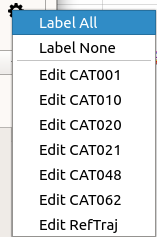
\includegraphics[width=3cm,frame]{figures/geoview_label_tab_menu.png}
  \caption{Geographic View Label Tab Menu}
\end{figure}

\subsubsection{Label Contents}

Using the 'Label menu' button \includegraphics[width=0.5cm,frame]{../../data/icons/edit.png}, the label content specific to a DBContent can be edited. \\

The label contents are organized in a 3x3 matrix, the contents if the first 2 rows and columns are fixed while row 3 and column 3 can be edited. 

\begin{figure}[H]
   \center
    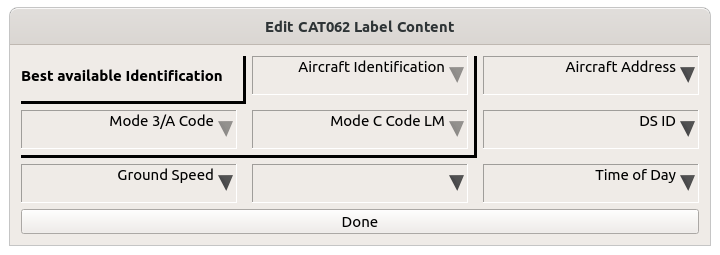
\includegraphics[width=14cm]{figures/geoview_label_content_edit.png}
  \caption{Geographic View Edit Label Contents}
\end{figure}

Multiple level of details (\textbf{LoD}s) are defined (as indicated with border lines in the edit dialog):
\begin{itemize}
 \item LoD 1: 1x1 matrix with the best available identification
 \item LoD 2: 2x2 matrix, LoD 1 with the most important secondary information
 \item LoD 3: 3x3 matrix, LoD 2 with some additional information
\end{itemize} 
\ \\

\begin{itemize}
\item LoD 1
\begin{itemize}
 \item Row 1, column 1: Best available indentification in bold text, in the following order
 \begin{itemize}
 \item Aircraft Identification, Aircraft Address, Mode 3/A Code, or '?' if not available
 \end{itemize} 
 \end{itemize} 
\item LoD 2 
 \begin{itemize}
 \item Row 1, column 2: Aircraft Identification
 \item Row 2, column 1: Mode 3/A Code
 \item Row 2, column 2: Mode C Code in flight levels
 \end{itemize} 
\item LoD 3
 \begin{itemize}
 \item Row 1, column 3: Aircraft Address
 \item Row 2, column 3: Data source ID
 \item Row 3, column 1: Ground Speed
 \item Row 3, column 2: empty by default
 \item Row 3, column 3: Time of Day
 \end{itemize} 
\end{itemize} 
\ \\

Please note that the Mode A and the Mode C code are automatically displayed using the respective garbled/valid flag information as suffixes:

\begin{itemize}
 \item (I)nvalid
 \item (G)arbled
 \item (S)moothed
\end{itemize} 

\subsubsection{Automatic Labeling}

If a data source to be labeled is activated, automatic labels are generated (into the configurated direction) and updated once per second. \\

Please \textbf{note} that when automatic labeling is active, manually created labels are removed once per second. This will be improved in the future.

\begin{figure}[H]
    \hspace*{-2.5cm}
    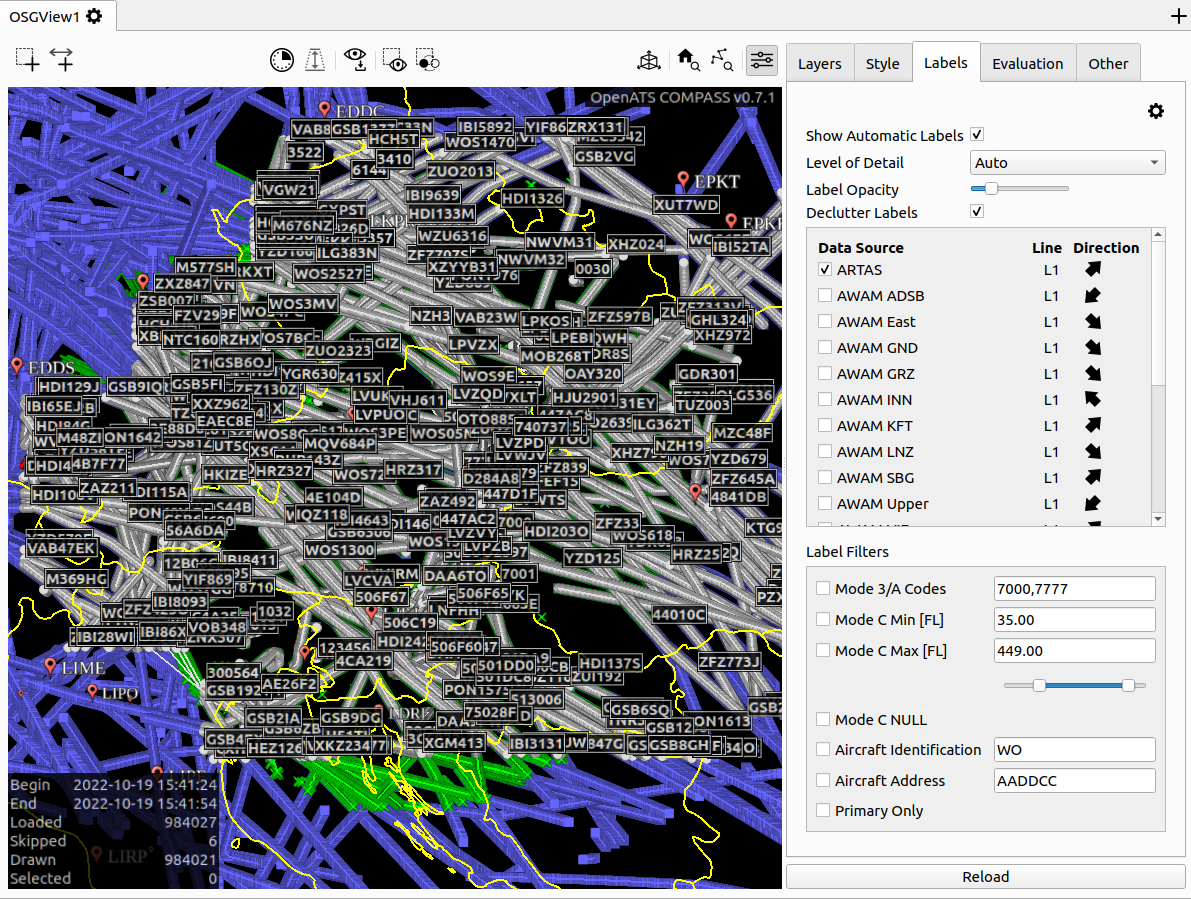
\includegraphics[width=19cm,frame]{figures/geoview_label_lod1.png}
  \caption{Geographic View Auto-Labels LoD 1}
\end{figure}

For each target (as in the the last layer item according to \nameref{sec:layer_mode}) a single label is created for the latest shown target report. \\

The Level of Detail can have the following values:
\begin{itemize}
 \item Auto: Automatic label size depending on number of visible labels
 \item LoD 1: 1x1 matrix
 \item LoD 2: 2x2 matrix
 \item LoD 3: 3x3 matrix
\end{itemize} 
\ \\

Depending on the number of visible labels, the LoD is chosen by Auto LoD, if (e.g. with zoom or time window filter operations) the number of visible labels is reduced, a higher LoD is shown.

\begin{figure}[H]
    \hspace*{-2.5cm}
    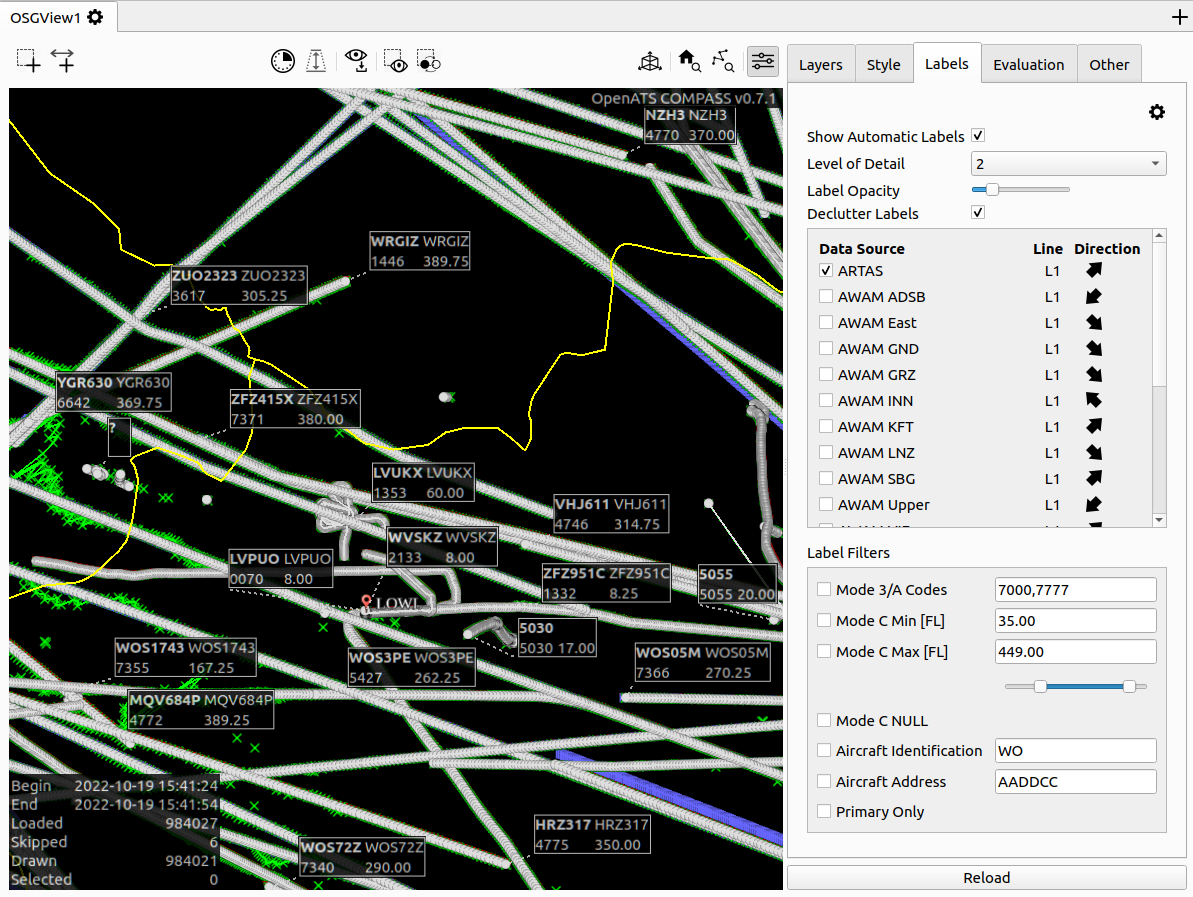
\includegraphics[width=19cm,frame]{figures/geoview_label_lod2.png}
  \caption{Geographic View Auto-Labels LoD 2}
\end{figure}

The automatic labeling can be most useful when choosing a target-specifc layer mode (e.g. based on unique secondary identification or UTN) and activating the time window filter (or in Live mode).

\begin{figure}[H]
    \hspace*{-2.5cm}
    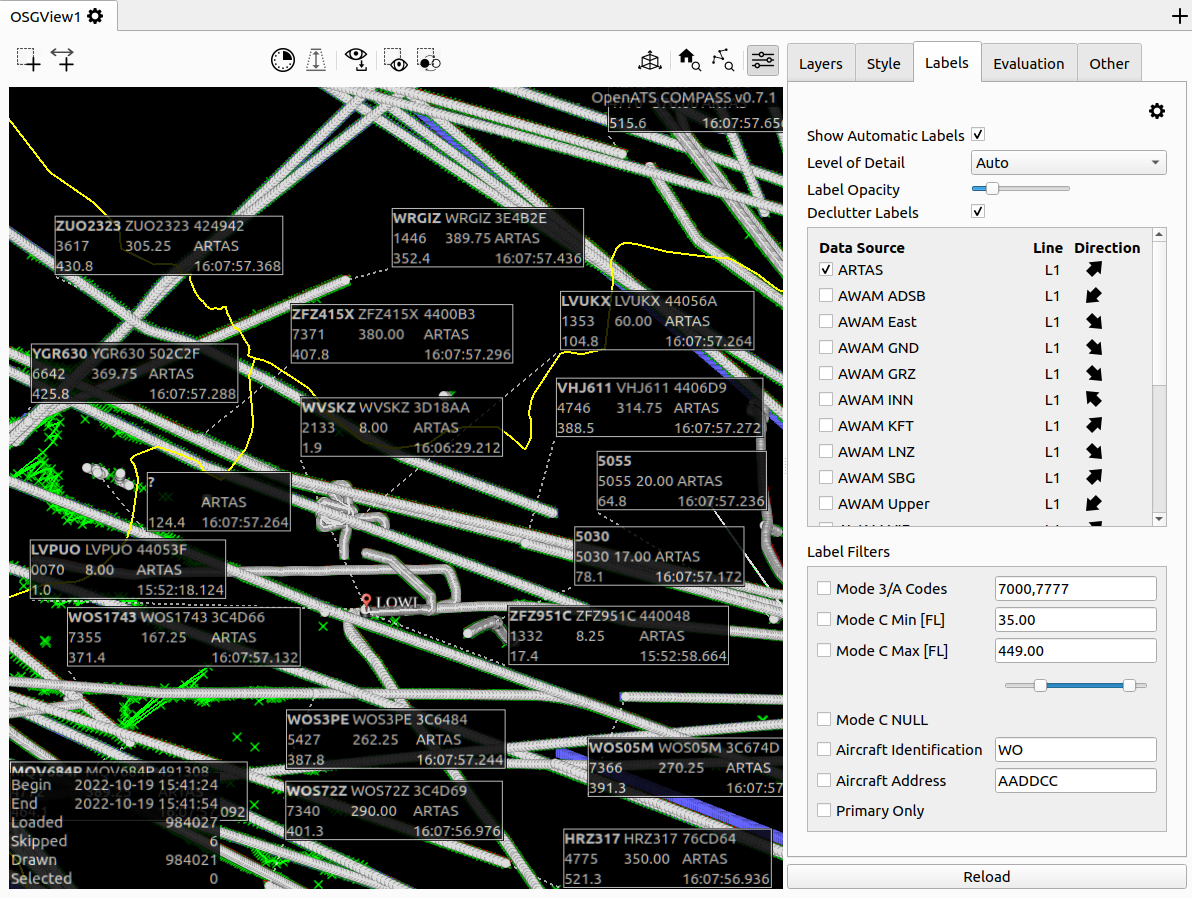
\includegraphics[width=19cm,frame]{figures/geoview_label_lod3.png}
  \caption{Geographic View Auto-Labels LoD 3}
\end{figure}


\subsubsection{Label Filters}

When automatic labeling is activated, labeling of targets can be restricted using the label filters. Each filter can be activated and its filter value set to label only targets with specific attributes. The filters offer similar ways as the ones defined in \nameref{sec:filters}.

\paragraph{Mode 3/A Codes}

When active, this filter forces labeling of data with the given Mode A code(s), so it is possible to give multiple values (in octal notation, separated by commas). E.g. '7000' is possible, or '7000,7777'. Target reports without a given Mode A will not be labeled unless the value 'NULL' is (also) given. \\

\paragraph{Mode C}

When active, based on the Mode C Min and Mode C Max values, target reports are only labeled if the minimum and maximum flight level matches the specified thresholds. Target reports without a Mode C Code will not be labeled unless the NULL checkbox is checked.

\paragraph{Aircraft Identifcation}

When active, this filter forces labeling of data only from aircraft identifications matching the given expression. The percent operator denotes a 'any characters' placeholder. So e.g. '\%TEST\%' will match 'TEST123' or 'TEST123   ' (with spaces) or 'MYTEST'. Target reports without a given aircraft identification will not be labeled unless the value 'NULL' is (also) given.


\paragraph{Aircraft Address}

When active, this filter forces labeling of the given Mode S address(es), so it is possible to give multiple values (in hexadecimal notation, irrespective of upper or lower case characters, separated by commas). E.g. 'FEFE10' is possible, or 'FEFE10,FEFE11,FEFE12'. Target reports without a given Mode S address will not be labeled unless the value 'NULL' is (also) given.



